\chapter{高次元エクスパンダー}
高次元エクスパンダーとはグラフのエクスパンダー性を単体複体に拡張した概念である.
\section{定義}
まずは単体複体に関する基礎的な用語を定義していく.
文脈によっては単体複体は多面体などを貼り合わせた幾何的な概念を指すこともあるが,
本講義では組合せ的ないわゆるset systemとしての単体複体を扱う.

\begin{definition}{単体複体}{simplicial complex}
有限集合$V$と$V$の部分集合族$\F\subseteq 2^V$であって部分集合で閉じているもの(すなわち, $\sigma\subseteq \tau \in \F \Rightarrow \sigma\in \F$)の組$X=(V,\F)$を\emph{単体複体 (simplicial complex)}という.
集合族$\F$の元を\emph{面 (face)}と呼び,
面$\sigma \in \F$の\emph{次元 (dimension)}を$\dim \sigma = \abs{\sigma} - 1$とする\footnote{特に, 空集合$\emptyset \in \F$の次元は$-1$である.}.
単体複体$X$の次元を$\dim X = \max\cbra{\dim \sigma \colon \sigma \in \F}$とする.

次元$d$の単体複体$X$は(包含関係に関して)極大な面の次元が全て$d$に等しいとき, \emph{純粋 (pure)}であるという.
整数$-1 \le k \le \dim X$に対し$X(k) = \cbra*{\sigma \in \F\colon \dim \sigma = k }$とする.
特に断りのない限り, $X(0)=V$を仮定する
(そうでなければ$V$として$V=X(0)$とした単体複体を考える).
\end{definition}
面の次元の概念は単体複体の幾何的な表現に由来する.
このイメージになぞらえて,
次元$0$の面を\emph{頂点 (vertex)}, 次元$1$の面を\emph{辺 (edge)}と呼ぶことがある.

\paragraph*{例1.}
グラフ$G=(V,E)$に対し, $\F = \{\emptyset\} \cup \cbra*{\{v\}\colon v \in V} \cup E$とすると, $(V,\F)$は単体複体である.
また, 次元$2$以上の任意の単体複体$X$に対して$(X(0),X(1))$はグラフである.

\paragraph*{例2.}
有限集合$V$に対し,
$\F = \binom{V}{\le k} \defeq \cbra*{ \sigma \subseteq V \colon |\sigma|\le k}$としたとき, $(V,\mathcal{F})$は純粋な$(k+1)$-次元の単体複体である.

\paragraph*{例3.}
閉路を含まないグラフを\emph{森 (forest)}といい, 連結な森を\emph{木 (tree)}という.
連結グラフ$G$の部分グラフであって木であるものを\emph{全域木 (spanning tree)}という.

グラフ$G=(V,E)$に対し,
森であるような部分グラフの辺集合からなる集合族$\F\subseteq 2^E$は単体複体である.
すなわち,
\begin{align*}
    \F = \cbra*{ F \subseteq E \colon \text{部分グラフ$(V,F)$は森}}
\end{align*}
に対して$(E,\F)$は単体複体である.
簡単のため$G$を連結グラフであるとすると, $(E,\F)$の極大面は$G$の全域木に対応し, その次元は$n-2$に等しい.
すなわち$(E,\F)$は純粋な$(n-2)$-次元単体複体である.

\paragraph*{例4.}
実行列$A\in \Real^{n\times m}$ (ただし$m\ge n$) の行ベクトルを$\vec{a}_1,\dots,\vec{a}_n$とする.
集合$V=\{1,\dots,n\}$の部分集合族であって, 線形独立な行ベクトル集合のインデックスとなるものの全体を$\F$とする.
すなわち
\[
    \F = \cbra*{ I \subseteq V\colon (\vec{a}_i)_{i\in I}\text{は線形独立}}
\]
とすると, $(V,\F)$は純粋な単体複体であり, その次元は$A$のランク$\mathrm{rank}(A)$に対し$\mathrm{rank}(A)-1$となる.

\paragraph*{例5.}
部集合$L,R$を持つ二部グラフ$G=(V,E)$を考える.
辺部分集合$M\subseteq E$は, 部分グラフ$(V,M)$の全ての頂点の次数が高々$1$であるとき\emph{マッチング (matching)}という.
マッチング$M$の部分集合$M'\subseteq M$もまたマッチングであるため,
グラフ$G$のマッチング全体からなる辺部分集合族$\F\subseteq 2^E$に対し, $(E,\F)$は単体複体である.
一般に極大マッチングのサイズは異なる場合があるのでこの単体複体は純粋ではない (\cref{fig:matching}).
\begin{figure}[htbp]
    \begin{center}
        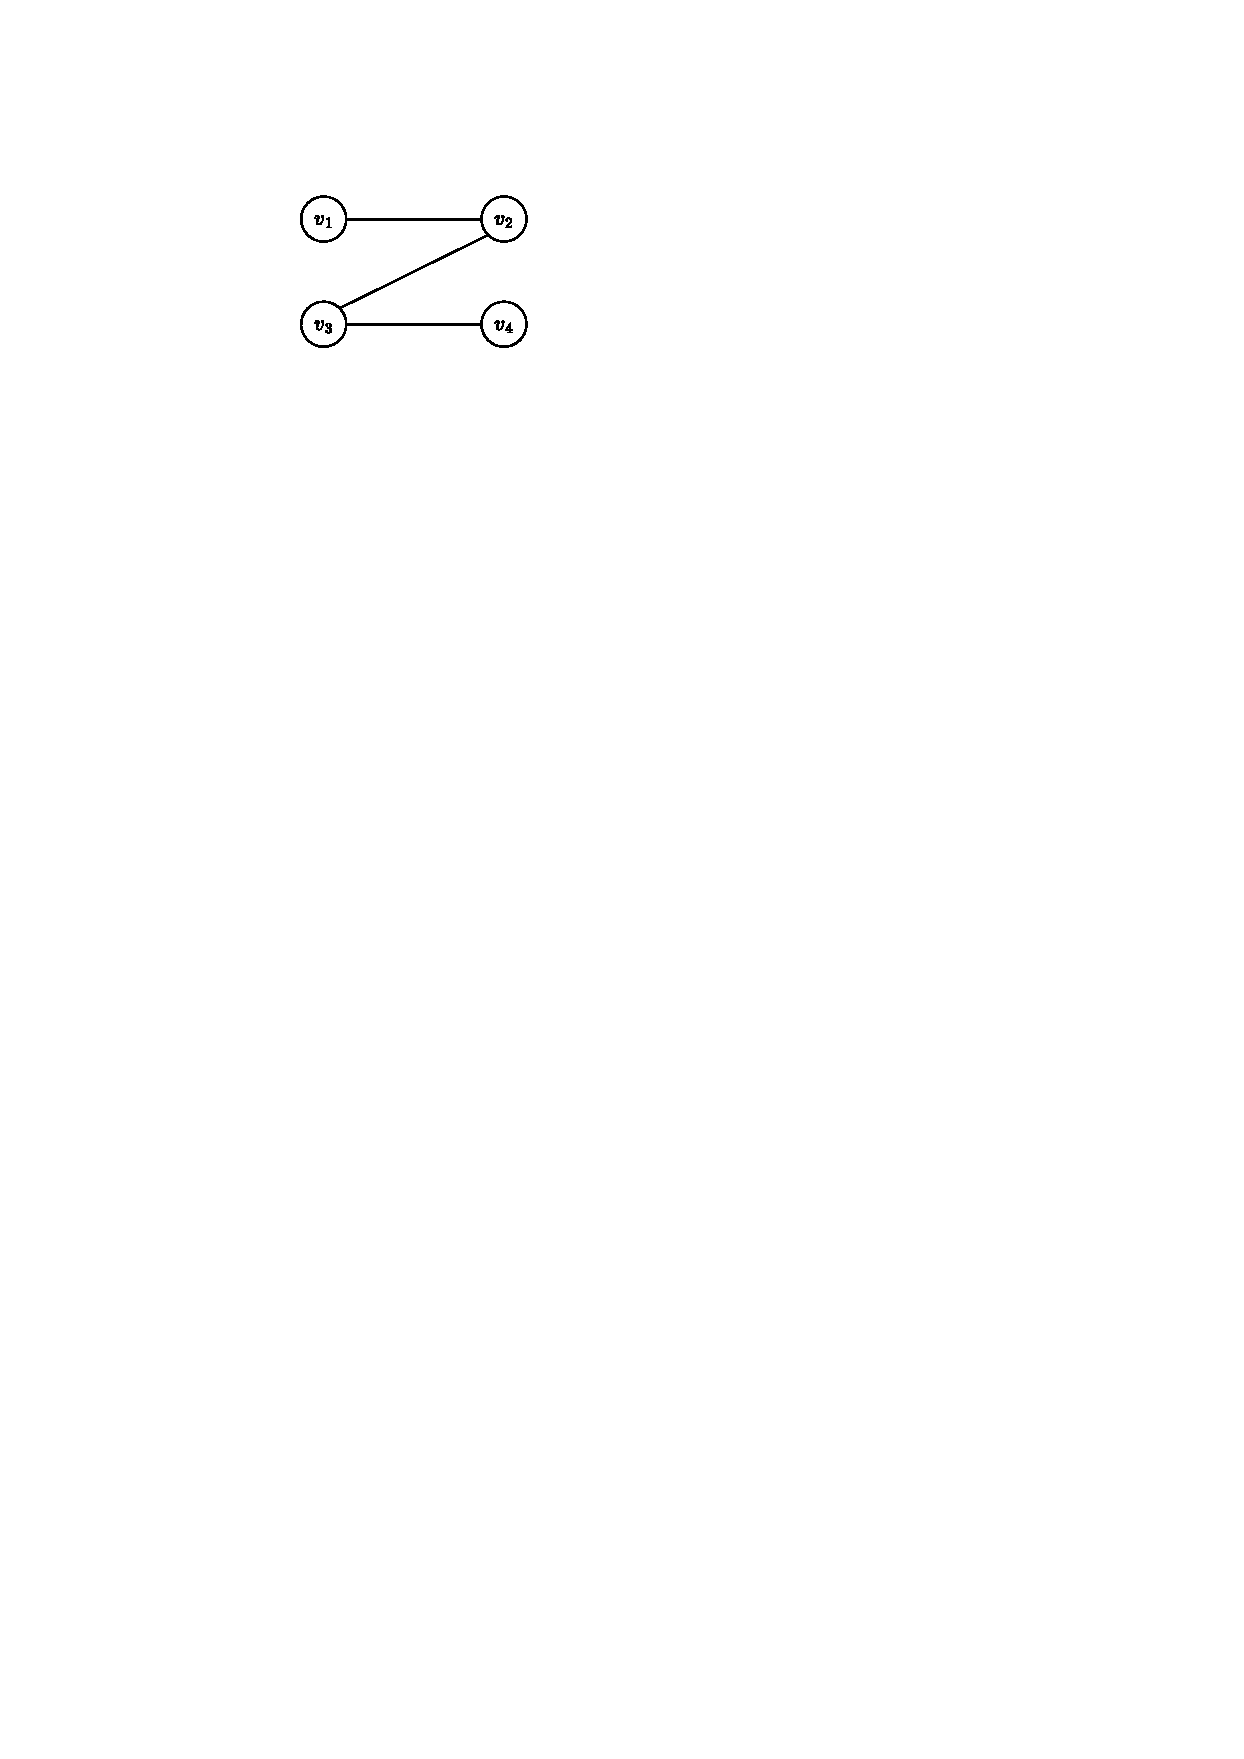
\includegraphics[width=5cm]{images/matching.pdf}
    \end{center}
    \caption{マッチング$M_1=\{v_1,v_2\},\{v_3,v_4\}\}$と$M_2=\{\{v_2,v_3\}\}$はどちらも極大である. \label{fig:matching}}
\end{figure}

\begin{definition}{リンクとスケルトン}{link and skelton}
    単体複体$X=(V,\F)$を考える.
    面$\sigma \in \F$の\emph{リンク (link)}とは単体複体$(V\setminus \sigma, \F_{\sigma})$であって集合族$\F_\sigma$が
    \[
        \F_\sigma = \cbra*{ \tau \setminus \sigma \colon \sigma \subseteq \tau \in \F }
    \]
    で与えられるものである.
    次元$k$以下の面の集合
    \[
        \F_k = \cbra*{ \sigma \in \F \colon \dim \sigma \le k}
    \]
    に対し$(V,\F_k)$を\emph{$k$-スケルトン ($k$-skelton)}という.
\end{definition}

%\end{definition}


\section{単体複体上のランダムウォーク}
グラフ上のランダムウォークは頂点集合上で遷移するものを考えていたが,
単体グラフ上のランダムウォークは同じ次元の面の間で遷移するものを考える.
アイデアとしては, \cref{sec:graph up and down walk}で考えたようにある次元$k$の面から次元$k+1$の面に遷移する上昇ウォークと逆に次元$k+1$の面から次元$k$の面に遷移する下降ウォークを組み合わせることによって, $X(k)$上のランダムウォークを定義する.

\begin{definition}{上昇ウォークと下降ウォーク}{up and down walk}
    純粋な$d$次元単体複体$X=(V,\F)$を考える.
\end{definition}
\section{局所スペクトルエクスパンダー}
\section{Oppenheimのトリクルダウン定理}
